En esta sección, se presentan los resultados obtenidos al reproducir cada uno de
los experimentos de la sección anterior, es decir, los experimentos que los autores
presentan en su trabajo \cite{jsantos-amonteagudo-1-2014}.

Antes de todo, hay que tener en cuenta la componente aleatoria de la simulación. Esto es, por
la realización de sorteos de cara a ejecutar la mitosis u otra acción. En consecuencia, la aparición
de un marcador u otro, como se verá a continuación, provoca alteraciones en la simulación, de modo que
el comportamiento puede variar. En este caso, lo que se pretende es llegar a la misma conclusión que los autores,
por tanto, el análisis de los resultados propios debe hacerse con ese objetivo en mente.

\section{Influencia del parámetro \textit{Tasa de mutación base (m)}}

Las células de la simulación, y como se ha descrito en secciones previas, tienen asociado una propiedad que está relacionada con la aparición
de nuevas mutaciones durante la mitosis, este es, el parámetro \textit{tasa de mutación base} o $m$. En este experimento,
se pretende someter a la simulación a diferentes configuraciones de este parametros para estudiar qué
progresión presentan los tumores.

Se parte de una probabilidad de aparición de mutaciones baja, ya que, el sorte se efectua con una probabilidad de
$1/m$, por lo que, a mayor valor del parámetro $m$, menor probabilidad de que ocurre. En este caso, se
realizan tres simulaciones, para $m=10000$, $m=1000$ y $m=100$.

\subsection{Experimento 1: Tasa de mutación base igual a 10.000}

En esta simulación, se obtienen tres gráficas respecto de la misma. En la primera, se observa la progresión
en el número de células sanas frente a células cancerosas.

En cuanto al número de células de uno u otro tipo, se observa una progresión bastante similar a la obtenida por los autores.
Por un lado, el número de células sanas crece muy rápido y ocupa el $90\%$ del espacio en torno a las $300$ iteraciones. Por otro lado,
el número de células cancerosas presenta una progresión similar con un repunte leve en torno a la iteración $300$ con un crecimiento muy leve.

\begin{figure}[h]
\centering
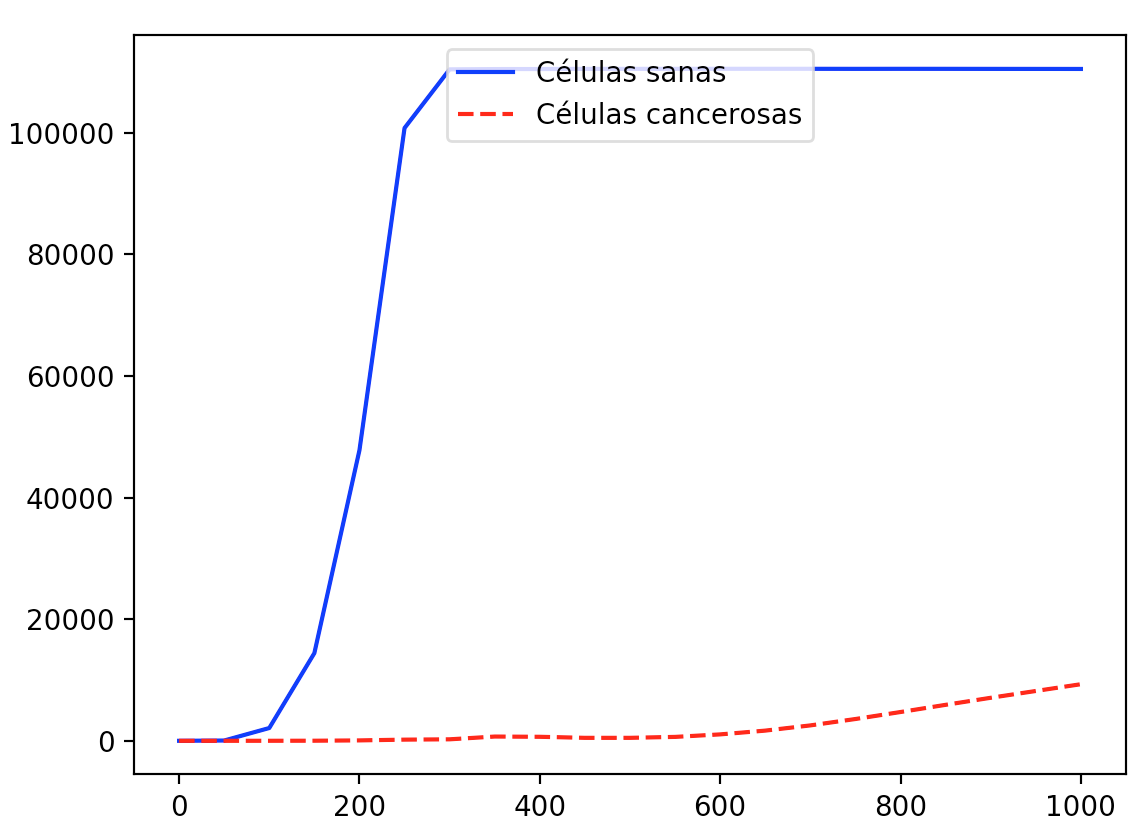
\includegraphics[scale=0.6]{figures/experiments/exp1/healthvscarcino}
\caption{Células sanas frente a células cancerosas como resultado de la simulación para el experimento con $m = 10,000$.}
\end{figure}

En cuanto a los marcadores presentes y a su progresión, se observan algunas diferencias. En primer lugar, el marcador
$SG$ toma ventaja respecto al resto, hasta que en torno a la iteración $500$ aproximadamente
también toma relevancia el marcador $EI$. Esto es especialmente relevante, e incluso, coherente con la simulación de los
propios autores.

El marcador $SG$ tiene una leve caída que se ve frenada cuando aparece el marcador $EI$. Este último, provoca
que las células puedan evitar la muerte celular o apoptosis. Esto hace que el marcador $SG$ tenga mayor presencia
y que el número de células vaya aumentando.

Se produce la peculiaridad de que ambas mutaciones, $SG$ y $EI$ se dan en las mismas células. Esto, como se observa
en la gráfica anterior, no tiene por qué afectar al número total de células cancerosas.

\begin{figure}[h]
\centering
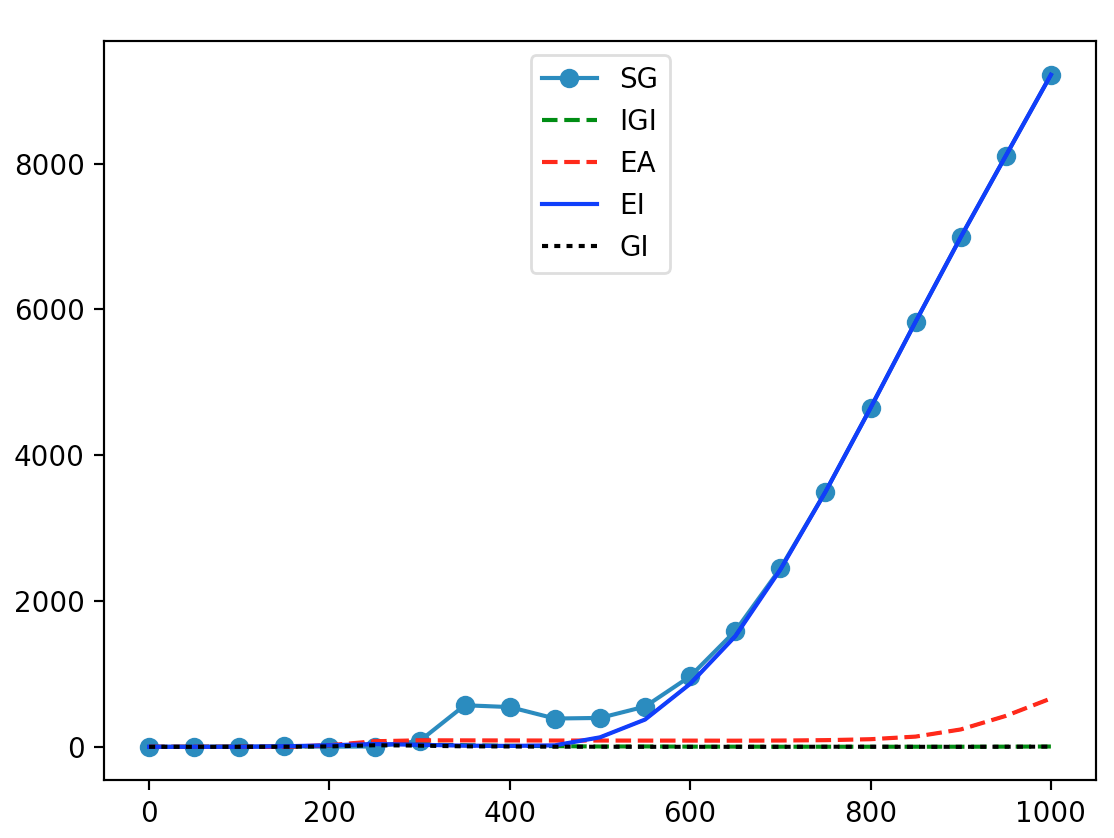
\includegraphics[scale=0.6]{figures/experiments/exp1/mutations}
\caption{Evolución de los marcadores como resultado de la simulación para el experimento con $m = 10,000$.}
\end{figure}

Por último, se muestra una vista de la rejilla, marcando las células cancerosas en verde. Tiene aspecto de estar completamente
ocupado por células cancerosas, pero esto es un efecto visual. Las células encuentran cabida en los límites de la rejilla
al haber obtenido el marcador $SG$, el cual permite ejecutar la mitosis más allá del espacio predefinido con suficiente
factor de crecimiento.

En la simulación de los autores se observa este mismo comportamiento. Esto es, por tanto, otro punto que es coherente con
los que presentan los autores en su estudio.

\begin{figure}[h]
\centering
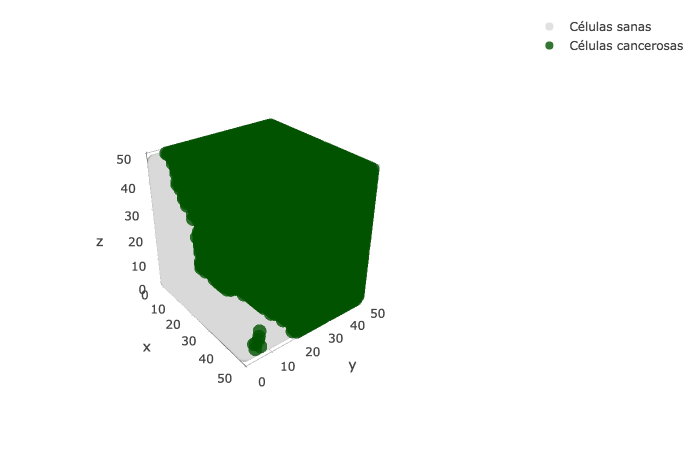
\includegraphics[scale=0.6]{figures/experiments/exp1/grid}
\caption{Rejilla resultante de la simulación para el experimento con $m = 10,000$.}
\end{figure}

\subsection{Experimento 2: Tasa de mutación base igual a 1.000}

El segundo experimento sobre el parámetros \textit{tasa de mutación base} se
mantienen todos los parámetros y se cambia dicho parámetro a $m=1000$.

Al igual que antes, se muestran tres gráficas. En la primera de ellas, que muestra la progresión de
células sanas frente a células cancerosas, se observa un comportamiento similar al obtenido
por los autores. Es decir, aparición de células cancerosas en torno a la iteración $150$,
crecimiento moderado, aunque algo mayor, lo que se explica por una mayor
probabilidad de aparición de mutaciones durante la mitosis. Al finalizar la simulación, se
observa algo más de $17000$ células cancerosas frente a unas $20000$ que obtienen los autores.

\begin{figure}[h]
\centering
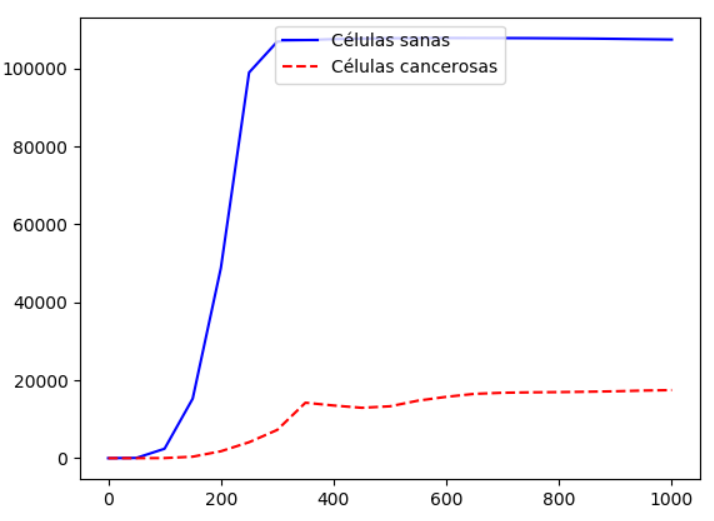
\includegraphics[scale=0.8]{figures/experiments/exp2/healthvscarcino}
\caption{Células sanas frente a células cancerosas como resultado de la simulación para el experimento con $m = 1,000$.}
\end{figure}

En cuanto a los marcadores, su progresión es diferente. En las primera $250$ iteraciones
el comportamiento es similar al obtenido por los autores, el primer marcador en tomar ventaja es
$EA$ y justo despues se ve superado por $SG$. La principal diferencia es que en torno a la iteración $450$
el marcador $EI$ aparece y tiene un crecimiento fuerte colocandose como el segundo marcador que más relevancia
toma.

Como se ha descrito, la aparición de los marcadores se realiza en base a una serie de sorteos con una probabilidad dada.
No se puede controlar su aparición. Lo relevante es que el resto de marcadores, $IGI$ y $GI$, casi no tienen relevancia
ni presencia.

Es decir, se obtiene un comportamiento parecido en cuanto a número de células sanas contra células cancerosas pero
con diferente presencia de marcadores. Esto quiere decir que los marcadores que más ventaja toman son los que realmente
afectan a la simulación. En este caso, obtener el marcador $EI$ hace que perduren las células que cuentan con dicha
mutación en su genoma y que se extienda en posteriores divisiones.

\begin{figure}[h]
\centering
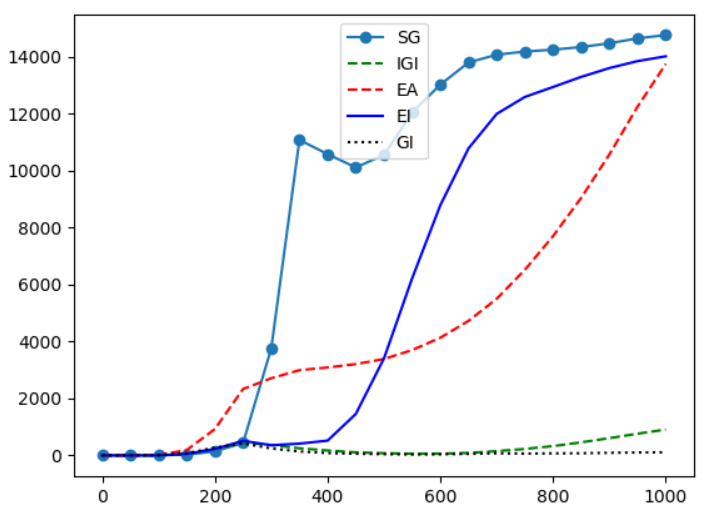
\includegraphics[scale=0.8]{figures/experiments/exp2/mutations}
\caption{Evolución de los marcadores como resultado de la simulación para el experimento con $m = 1,000$.}
\end{figure}

En cuanto a la rejilla, al igual que los resultados presentados por los autores, las células cancerosas
tienden a ocupar los límites de la rejilla, esto es devido a la pronta aparición del marcador $SG$. Las células con
otro tipo de marcadores tienden a encontrarse más hacia el centro de la rejilla.

\begin{figure}[h]
\centering
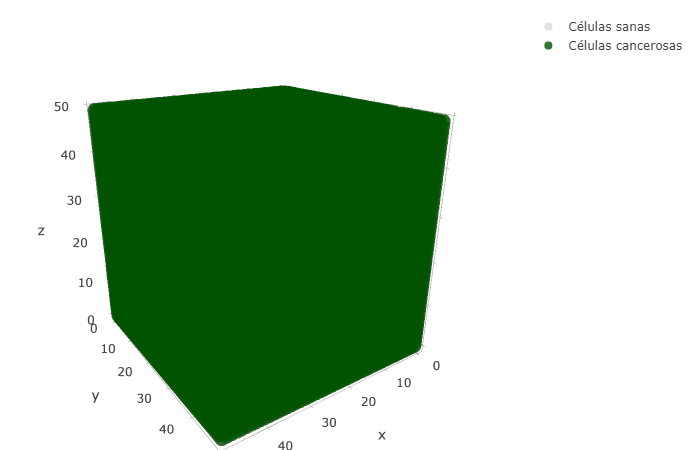
\includegraphics[scale=0.6]{figures/experiments/exp2/grid}
\caption{Rejilla resultante de la simulación para el experimento con $m = 10,000$.}
\end{figure}

\subsection{Experimento 3: Tasa de mutación base igual a 100}

En este último experimento para el parámetros \textit{tasa de mutación base}, se
quiere aumentar la probabilidad de que se produzcan mutaciones durante la mitosis.

En cuanto a células sanas frente a células cancerosas se observa como a lo largo de la simulación la
tendencia es que las células cancerosas van tomando relevancia frente a las células sanas. Los autores
observan que las células cancerosas superan a las sanas en torno a la iteración $180$ aproximadamente.
En este caso, en la simulación propia no se llega a ese resultado, pero si se observa una tendencia esperada,
y es que las células cancerosas superen en algún punto a las células sanas.

\begin{figure}[h]
\centering
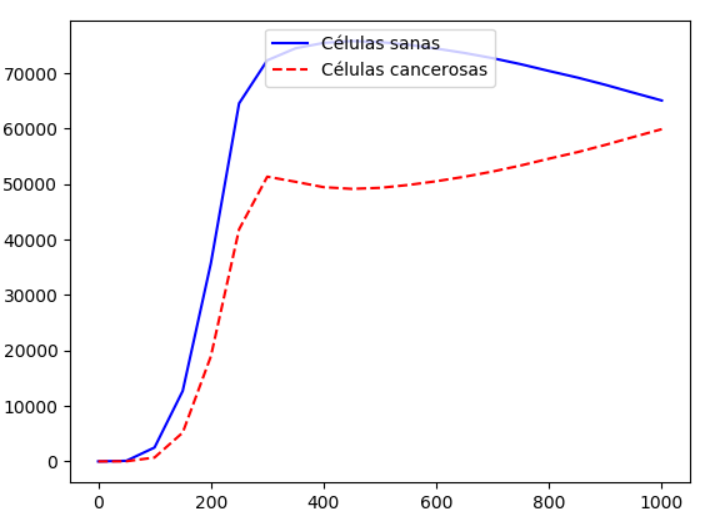
\includegraphics[scale=0.8]{figures/experiments/exp3/healthvscarcino}
\caption{Células sanas frente a células cancerosas como resultado de la simulación para el experimento con $m = 100$.}
\end{figure}

En cuanto a las mutaciones, al igual que los autores el marcador $EA$ es el más relevante, aunque lo hace
con mayor diferencia. Esto puede explicar la diferencia de comportamiento frente a lo mostrado anteriormente.
El marcador $IGI$ va tomando ventaja al final de la simulación, y no desde un principio como si ocurre en
la simulación de los autores.

Es relevante como el marcador $GI$ en todas las simulaciones no toma relevancia.

\begin{figure}[h]
\centering
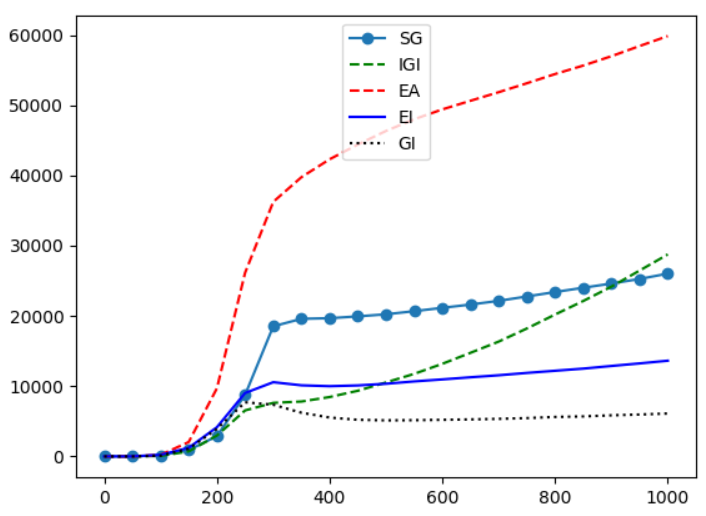
\includegraphics[scale=0.8]{figures/experiments/exp3/mutations}
\caption{Evolución de los marcadores como resultado de la simulación para el experimento con $m = 100$.}
\end{figure}

En cuanto a la posición de las células cancerosas en la rejilla, las conclusiones son las mismas
que en los dos experimentos anteriores, con mayor presencia de células cancerosas en la parte central
de la rejilla, lo que es coherente con lo que han obtenido los autores.

\begin{figure}[h]
\centering
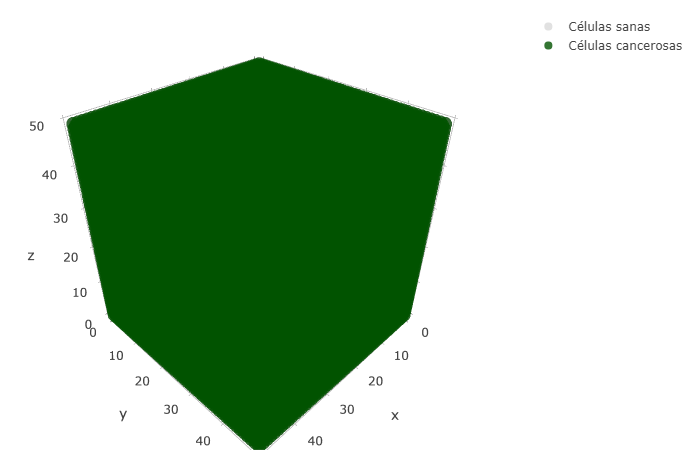
\includegraphics[scale=0.6]{figures/experiments/exp3/grid}
\caption{Rejilla resultante de la simulación para el experimento con $m = 100$.}
\end{figure}
